\documentclass{article}
\newcommand\tab[1][1cm]{\hspace*{#1}}
\usepackage[margin=60pt]{geometry}
\usepackage{hyperref}
\usepackage{makeidx}
\graphicspath{{./res/}}
\makeindex
\begin{document}
\begin{titlepage}
   \vspace*{\stretch{1.0}}
   \begin{center}
      \Huge\textbf{Progetto reti logiche}\\
      \vspace{5mm} %5mm vertical space
      \Large Prof. Gianluca Palermo - Anno 2019/2020\\
      \vspace{5mm} %5mm vertical space
      \large\textit{Rigutti Luca [codice persona: 10558383]}
      \linebreak
      \large\textit{Tortorelli Giuseppe [codice persona: 10582962]}
   \end{center}
   \vspace*{\stretch{2.0}}
\end{titlepage}
\printindex

\tableofcontents
\pagebreak

\section{Introduzione}
\subsection{Scopo del progetto}
Il progetto di reti logiche dell'anno accademico 2019-2020 si basa sul metodo di codifica a bassa dissipazione di potenza detto "Working Zone".
Il metodo Working Zone lavora sul Bus Indirizzi e si usa per codificare il valore di un indirizzo nel caso questo appartenga a certi intervalli noti, le working-zone. Ci possono essere multiple working-zone, ognuna delle quali parte da un indirizzo base e si estende per una dimensione fissa.
\subsection{Specifiche generali}
Vengono fornite 8 Working Zone e l'indirizzo da codificare. Ogni Working Zone parte dall'indirizzo base e si estende per una dimensione complessiva di 4 indirizzi (incluso quello base).\\Si possono presentare due casi:
\begin{enumerate}
\item\textbf{Indirizzo non presente in nessuna Working Zone}\\
In questo caso l'indirizzo codificato da restituire in output è così formato:
\begin{center}
\textbf{WZ\_BIT} \& \textbf{ADDR}
\end{center}
\begin{itemize}
\item\textbf{WZ\_BIT}: è il bit che indica se l'indirizzo appartiene o meno a qualche Working Zone e in questo caso vale 0.
\item\textbf{ADDR}: è l'indirizzo originale fornito in input.
\end{itemize}
\item\textbf{Indirizzo presente in una Working Zone}\\
In questo caso l'indirizzo codificato da restituire in output è così formato:
\begin{center}
\textbf{WZ\_BIT} \& \textbf{WZ\_NUM} \& \textbf{WZ\_OFFSET}
\end{center}
\begin{itemize}
\item\textbf{WZ\_BIT}: è il bit che indica se l'indirizzo appartiene o meno a qualche Working Zone e in questo caso vale 1.
\item\textbf{WZ\_NUM}: è il numero della Working Zone a cui l'indirizzo appartiene.
\item\textbf{WZ\_OFFSET}: è l'offset tra l'indirizzo base della Working Zone e l'indirizzo da codificare.
\end{itemize}
\end{enumerate}
L'indirizzo da codificare è espresso su 7 bit, in modo tale da rappresentare tutti i valori che vanno da 0 a 127. Le Working Zone e l'indirizzo codificato sono espressi su 8 bit.\\\\
Poichè le Working Zone sono 8, WZ\_NUM è espresso su 3 bit. Ne consegue che WZ\_OFFSET è espresso su 4 bit.\\
In particolare WZ\_OFFSET è codificato 1 hot così come segue:
\begin{itemize}
\item WZ\_OFFSET = 0 è codificato come 0001;
\item WZ\_OFFSET = 1 è codificato come 0010;
\item WZ\_OFFSET = 2 è codificato come 0100;
\item WZ\_OFFSET = 3 è codificato come 1000;
\end{itemize}
\pagebreak
\subsection{Interfaccia del componente}
{\fontfamily{qcr}\selectfont
entity poject\_reti\_logiche is\\
\tab port (\\
\tab\tab i\_clk\hspace*{1,5cm} : in std\_logic;\\
\tab\tab i\_start\hspace*{1,1cm} : in std\_logic;\\
\tab\tab i\_rst\hspace*{1,5cm} : in std\_logic;\\
\tab\tab i\_data\hspace*{1,3cm} : in std\_logic\_vector(7 downto 0);\\
\tab\tab o\_address\hspace*{0,7cm} : out std\_logic\_vector(15 downto 0);\\
\tab\tab o\_done\hspace*{1,3cm} : out std\_logic;\\
\tab\tab o\_en\hspace*{1,7cm} : out std\_logic;\\
\tab\tab o\_we\hspace*{1,7cm} : out std\_logic;\\
\tab\tab o\_data\hspace*{1,3cm} : out std\_logic\_vector(7 downto 0)\\
\tab );\\
end project\_reti\_logiche;
}
\begin{itemize}
\vspace{5mm} %5mm vertical space
\item i\_clk è il segnale di CLOCK;
\item i\_start è il segnale di START;
\item i\_rst è il segnale di RESET;
\item i\_data è il segnale che arriva dalla memoria in seguto ad una richiesta di lettura;
\item o\_address è il segnale di uscita che manda l'indirizzo alla memoria;
\item o\_done è il segnale di uscita che comunica la fine dell'elaborazione
\item o\_en è il segnale di ENABLE da mandare alla memoria per abilitare la lettura
\item o\_we è il segnale di WRITE ENABLE da mandare alla memoria per abilitare la scritture
\item o\_data è il segnale di uscita che invia alla memoria l'indirizzo codificato
\end{itemize}
\pagebreak
\subsection{Dati e descrizione memoria}
I dati, ciascuno di dimensione 8 bit (ADDR è esteso con uno 0 in posizione più significativa), sono memorizzati in una memoria RAM di 16 celle con indirizzamento al byte:
\begin{itemize}
\item Le cella di indirizzi dallo 0 al 7 contengono gli indirizzi base delle 8 Working Zone;
\item La cella di indirizzo 8 contiene l'indirizzo da codificare;
\item La cella di indirizzo 9 contiene l'indirizzo codificato che viene fornito in output;
\item Le restanti celle sono inutilizzate;
\end{itemize}
\begin{figure}[h]
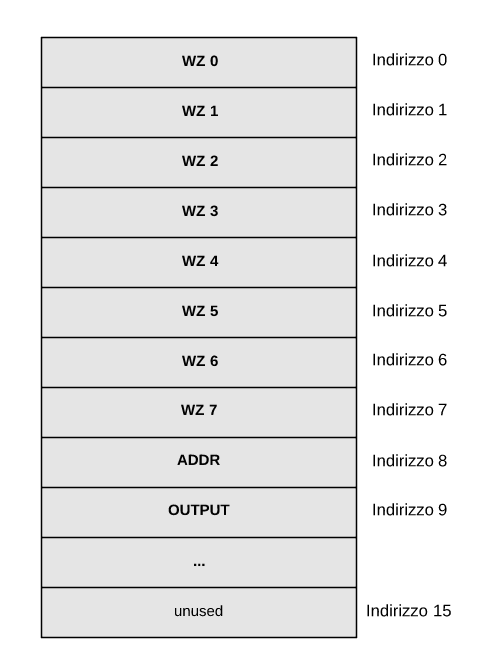
\includegraphics{memoria.png}
\end{figure}
\section{Design}
\subsection{Stati della macchina}
\subsubsection{stato x}
Nella progettazione del sistema, visto che per accedere alla ram si può farlo solo un ciclo di clock alla volta, si è deciso di memorizzare le working zone all'interno del circuito per poter eseguire la codifica su un ciclo di clock per ogni indirizzo da codificare.
\section{Risultati dei test}
Qui mettiamo uno screenshot del simulatore
\section{Conclusione}
\subsection{Risultati della sintesi}
\subsection{Ottimizzazioni}
\end{document}
